

\section{Predictive Tasks as Graph Representation Learning Problems}\label{sec:formal_rl_problem}

Here, we formulate a generic machine learning architecture based on Graph Neural Networks, which solves predictive tasks on relational databases.
The following section will first introduce three important graph concepts, which are outlined in Fig.~\ref{fig:three_graphs}: (a) The \emph{schema graph} (\emph{cf.}~Sec.~\ref{sec:schema_graph}), table-level graph, where one table corresponds to one node. (b) The \emph{relational entity graph} (\emph{cf.} Sec.~\ref{sec:formal_rl_graph}), an entity-level graph, with a node for each entity in each table, and edges are defined via foreign-primary key connections between entities. (c) The \emph{time-consistent computation graph} (\emph{cf.}~Sec.~\ref{sec:temporal_sampling}), which acts as an explicit training example for graph neural networks.
We describe generic procedures to map between graph types, and finally introduce our GNN blueprint for end-to-end learning on relational databases (\emph{cf.}~Sec.~\ref{sec:task_specific_gnn}).

\begin{figure}[t] % 'h' for here
  \centering
   \centering
     \begin{subfigure}[b]{0.28\textwidth}
         \centering
         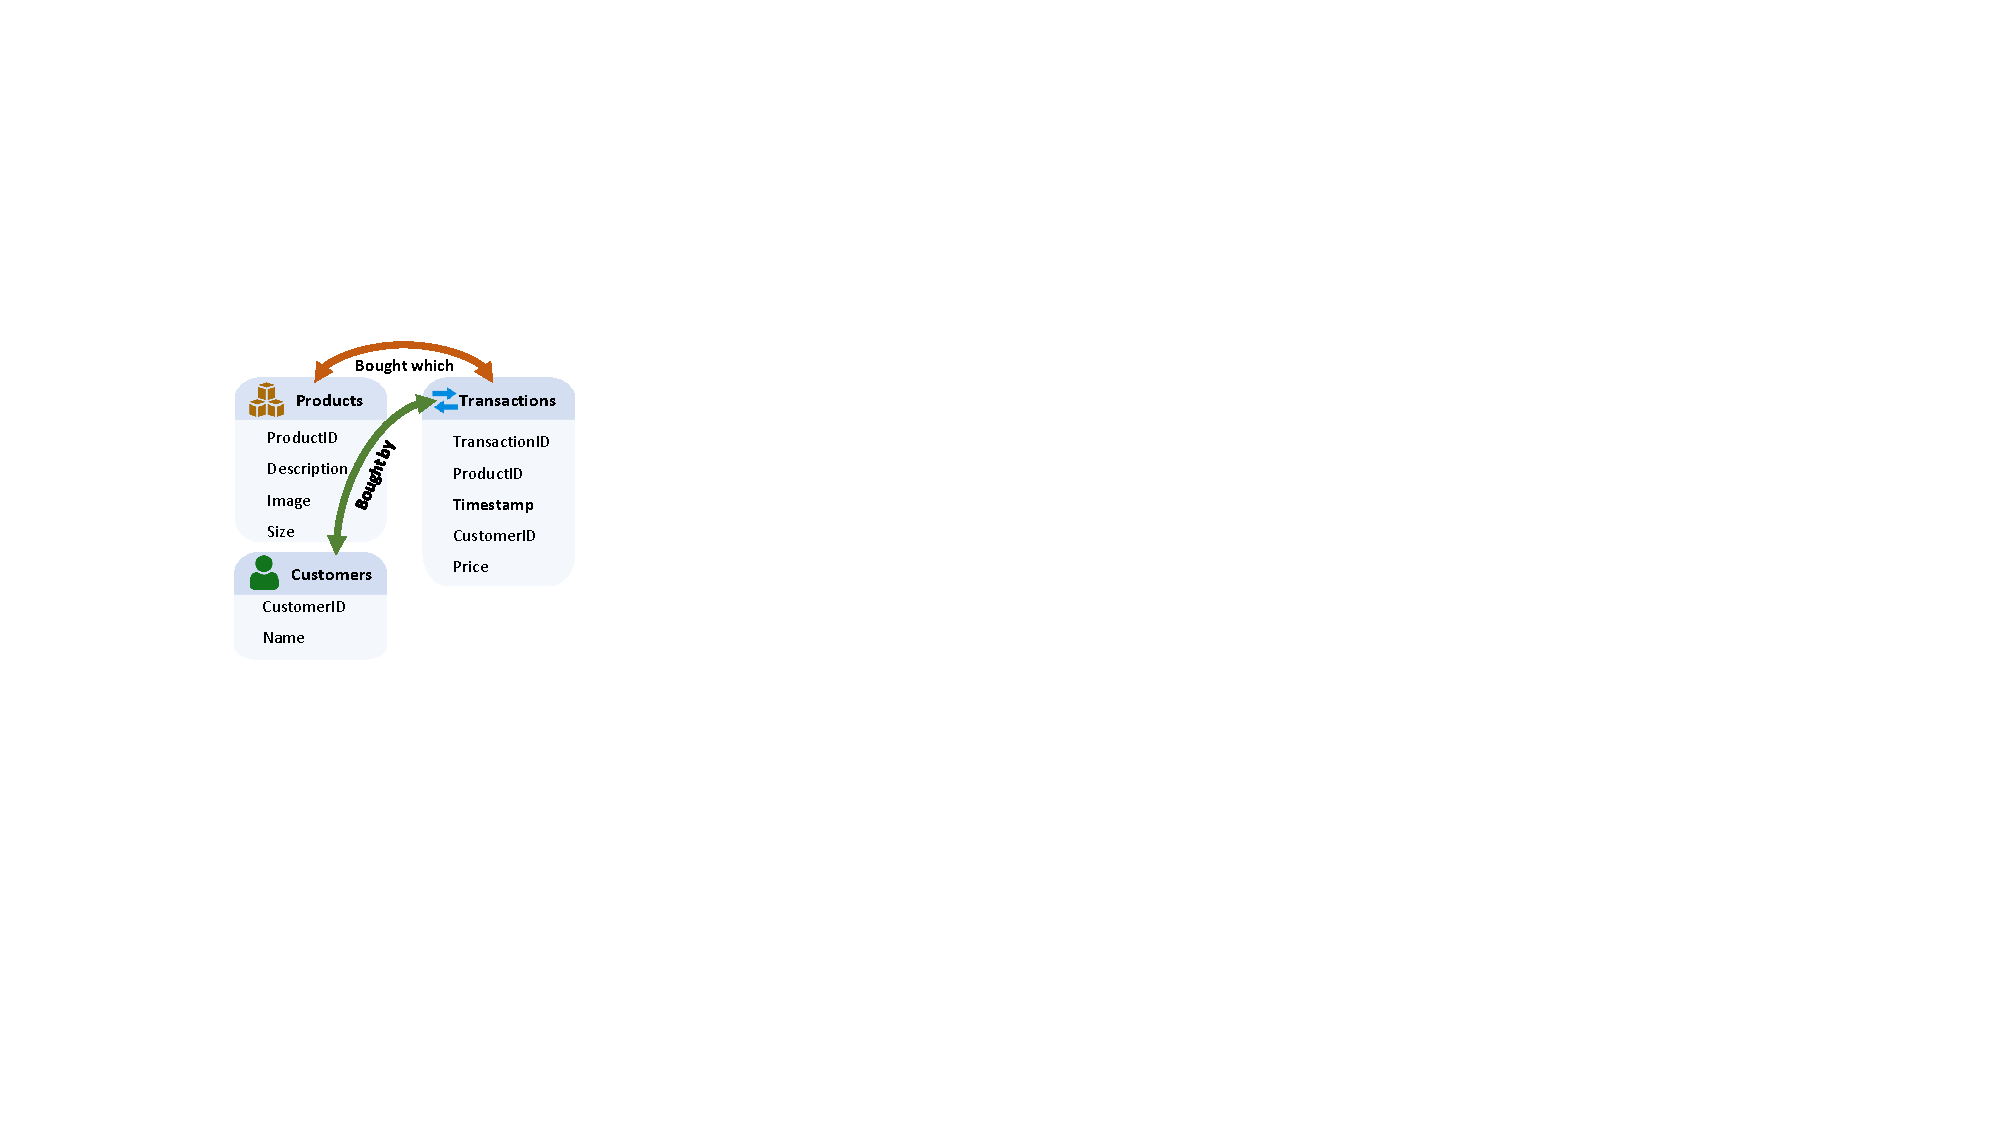
\includegraphics[width=\textwidth]{figs/f4a.pdf}
         \vspace{-0.6cm}
         \caption{Schema Graph}
         \label{fig:schema_graph}
     \end{subfigure}
     \hfill
     \begin{subfigure}[b]{0.27\textwidth}
         \centering
         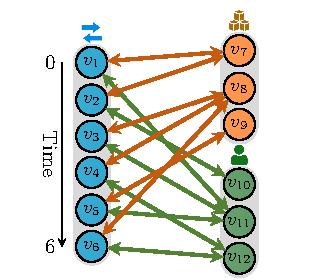
\includegraphics[width=\textwidth]{figs/tikz/graph2.pdf}
         \caption{Relational Entity Graph}
         \label{fig:instrinsic_data_graph}
     \end{subfigure}
     \hfill
     \begin{subfigure}[b]{0.43\textwidth}
         \centering
         %\vspace{0.1cm}
         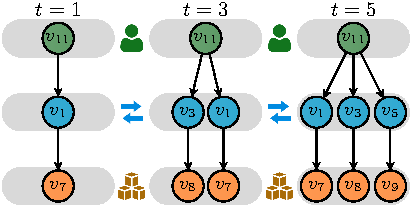
\includegraphics[width=\textwidth]{figs/tikz/graph3.pdf}
         %\vspace{0.001cm}
         \caption{Computation Graphs for different time $t$}
         \label{fig:example_graph}
     \end{subfigure}

  %\includegraphics[width=0.7\linewidth]{image-file-name} % Adjust width as needed
  \caption{\textbf{Three different kinds of graphs.} \textbf{(a)} The schema graph arises from the given relational tables. Each node denotes a table, and an edge between tables indicates that primary keys in one are foreign keys in the other. \textbf{(b)} The entity graph has one node for each entity in each table, and edges given by primary-foreign key links. The entity graph is heterogeneous with node and edge types defined by the schema graph. The nodes have a timestamp (illustrated by arrow-of-time), originating from the timestamp column of the table.
  \textbf{(c)} Using a temporal sampling strategy and a task description in form of training table containing different time $s$, we obtain \emph{time-consistent computation graphs} as training examples that naturally respect temporal order and map well to parallel compute.
  }
  \label{fig:three_graphs}
\end{figure}

\subsection{Schema Graph}
\label{sec:schema_graph}

The first graph in our blueprint is the \emph{schema graph} (\emph{cf.} Fig. \ref{fig:three_graphs}a), which describes the table-level structure of data.
Given a relational database $(\mathcal{T}, \mathcal{L})$ as defined in Sec.~\ref{sec: problem scope}, we let \mbox{$\mathcal L^{-1} = \{(T_{\rm pkey}, T_{\rm fkey}) \mid (T_{\rm fkey}, T_{\rm pkey}) \in \mathcal{L}\}$} denote its inverse set of links.
Then, the \emph{schema graph} is the graph $(\mathcal{T}, \mathcal{R})$ that arises from the relational database, with node set $\mathcal{T}$ and edge set $\mathcal{R} = \mathcal L \cup \mathcal L^{-1}$.
Inverse links ensure that all tables are reachable within the schema graph.
The schema graph nodes serve as type definitions for the heterogeneous relational entity graph, which we define next. 


\subsection{Relational Entity Graph}
\label{sec:formal_rl_graph}

To formulate a graph suitable for processing with GNNs, we introduce the \emph{relational entity graph}, which has entity-level nodes and serves as the basis of the proposed relational learning framework.

Our relational entity graph is a \emph{heterogeneous graph}  $G=(\mathcal{V}, \mathcal{E}, \phi, \psi)$, with node set $\mathcal{V}$ and edge set $\mathcal{E} \subseteq \mathcal V \times \mathcal V$ and type mapping functions $\phi: \mathcal{V} \rightarrow \mathcal{T}$ and $\psi: \mathcal{E} \rightarrow \mathcal{R}$, where each node $v \in \mathcal{V}$ belongs to a \emph{node type} $\phi(v) \in \mathcal{T}$ and each edge $e \in \mathcal E$ belongs to an \emph{edge type} $\psi(e) \in \mathcal{R}$.
Specifically, the sets $\mathcal{T}$ and $\mathcal{R}$ from the schema graph define the node and edge types of our relational entity graph.

Given a schema graph $(\mathcal{T}, \mathcal{R})$ with tables $T = \{v_1, ..., v_{n_T}\}\in\mathcal{T}$ as defined in Sec.~\ref{sec: problem scope}, we define the node set in our relational entity graph as the union of all entries in all tables $\mathcal{V} = \bigcup_{T\in\mathcal{T}}T$.
Its edge set is then defined as
\begin{equation}
\mathcal{E} = \{(v_1, v_2) \in \mathcal{V} \times \mathcal{V} \mid  p_{v_2} \in \mathcal{K}_{v_1} \text{ or } p_{v_1} \in \mathcal{K}_{v_v}\}\textnormal{,}
\end{equation}
\emph{i.e.} the entity-level pairs that arise from the primary-foreign key relationships in the database. 
We equip the relational entity graph with the following key information:
\begin{itemize}
    \item \textbf{Type mapping functions} $\phi: \mathcal{V} \rightarrow \mathcal{T}$ and $\psi: \mathcal{E} \rightarrow \mathcal{R}$, mapping nodes and edges to respective elements of the schema graph, making the graph \emph{heterogeneous}. We set $\phi(v) = T$ for all $v\in T$ and $\psi(v_1,v_2) = (\phi(v_1), \phi(v_2)) \in \mathcal R$ if $(v_1,v_2) \in \mathcal E$.
    \item \textbf{Time mapping function} $\tau: \mathcal{V} \rightarrow \mathcal{D}$, mapping nodes to its timestamp: $\tau: v \mapsto t_v$ (as defined in Sec.~\ref{sec:rel_dbs}), introducing time as a central component and establishes the \emph{temporality} of the graph. The value $\tau(v)$ denotes the point in time in which the table row $v$ became available or $-\infty$ in case of non-temporal rows.
    \item \textbf{Embedding vectors} $\mathbf{h}_v \in \mathbb{R}^{d_{\phi(v)}}$ for each $v\in\mathcal{V}$, which contains an embedding vector for each node in the graph. Initial embeddings are obtained via multi-modal column encoders as described in Sec.~\ref{sec:encoders}. Final embeddings are computed via GNNs outlined in Section 3.4.
\end{itemize}

An example of a relational entity graph for a given schema graph is given in Fig.~\ref{fig:instrinsic_data_graph}.
The graph contains a node for each row in the database tables. Two nodes are connected if the foreign key entry in one table row links to the primary key entry of another table row. Node and edge types are defined by the schema graph. Nodes resulting from temporal tables carry the timestamp from the respective row, allowing temporal message passing, which is described next.



\subsection{Time-Consistent Computational Graphs}
\label{sec:temporal_sampling}

Given a relational entity graph and a training table  (\emph{cf.}~Sec.~\ref{sec:predictive_labels}), we need to be able to query the graph at specific points in time which then serve as explicit training examples used as input to the model.
In particular, we create a subgraph from the relational entity graph induced by the set of foreign keys $\mathcal{K}_v$ and its timestamp $t_v$ of a training example in the training table $T_\text{train}$.
This subgraph then acts as a local and \emph{time-consistent computation graph} to predict its ground-truth label $y_v$.

\begin{algorithm}[t]
\caption{Time-Consistent Computation Graph}\label{alg:temp_sampling}
\begin{algorithmic}
\Require Relational entity graph $G = (\mathcal{V}, \mathcal{E})$, number of hops $L$, seed node $v_0\in\mathcal{V}$, seed time $t \in \mathbb{R}$
\Require Neighborhood sizes $(m_1,...,m_L) \in \mathbb{N}^L$
\Ensure Computation graph $G_{\rm comp} = (\mathcal{V}_{\rm comp}, \mathcal{E}_{\rm comp})$
\State $\mathcal V_0 \gets \{v_0\}$\textnormal{,} \quad $\mathcal E_0 \gets \emptyset $
\For{$i \in \{1,...,L\}$}
\For{$v \in \mathcal V_{i-1}$}
    \State $\mathcal{E}_i \gets \textnormal{SELECT}_{m_i}(\{(w,v) \in \mathcal{E} \mid \tau(v)\leq t\})$ \Comment{Select a maximum of $m_i$ filtered edges}
    \State $\mathcal{V}_i \gets \{w \in \mathcal{V} \mid (w,v) \in \mathcal{E}_i\}$  \Comment{Gather nodes for the sampled edges}
\EndFor
\EndFor
\State $\mathcal V_{\rm comp} \gets \bigcup_{i=1}^L \mathcal V_i$\textnormal{,} \quad $\mathcal E_{\rm comp} \gets \bigcup_{i=1}^L \mathcal E_i$
\end{algorithmic}
\end{algorithm}

The computational graphs obtained via neighbor sampling~\citep{hamilton2017inductive} allow the scalability of our proposed approach to modern large-scale relational data  with billions of table rows, while ensuring the temporal constraints~\citep{wang2021temporalsampling}.
Specifically, given a number of hops $L$ to sample, a seed node $v \in \mathcal{V}$, and a timestamp $t$ induced by a training example, the computation graph is defined as $G_{\rm comp} = (\mathcal{V}_{\rm comp}, \mathcal{E}_{\rm comp})$ as the output of Alg.~\ref{alg:temp_sampling}. 
The algorithm traverses the graph starting from the seed node $v$ for $L$ iterations. In iteration $i$, it gathers a maximum of $m_i$ neighbors available up to timestamp $t$, using one of three selection strategies:
\begin{itemize}
    \item \textbf{Uniform temporal sampling} selects uniformly sampled random neighbors.
    \item \textbf{Ordered temporal sampling} takes the latest neighbors, ordered by time $\tau$.
    \item \textbf{Biased temporal sampling} selects random neighbors sampled from a multinomial probability distribution induced by $\tau$. For instance, sampling can be performed proportional to relative neighbor time or biased towards specific important historical moments. 
\end{itemize}

The temporal neighbor sampling is performed purely on the graph structure of the relational entity graph, without requiring initial embeddings $\mathbf{h}^{(0)}_v$. The bounded size of computation graph $G_{\rm comp}$ allows for efficient mini-batching on GPUs, independent of relational entity graph size.
In practice, we perform temporal neighbor sampling on-the-fly, which allows us to operate on a shared relational entity graph across all training examples, from which we can then restore local and historical snapshots very efficiently.
Examples of computation graphs are shown in Fig.~\ref{fig:example_graph}.

\subsection{Task-Specific Temporal Graph Neural Networks}
\label{sec:task_specific_gnn} 

Given a time-consistent computational graph and its future label to predict, we define a generic multi-stage deep learning architecture as follows:
\begin{enumerate}
\setlength\itemsep{0em}
    \item Table-level \textbf{column encoders} that encode table row data into initial node embeddings $\mathbf{h}^{(0)}_v$, as described in Sec.~\ref{sec:encoders}.
    \item A stack of $L$ \textbf{relational-temporal message passing layers} (\emph{cf.}~Sec.~\ref{sec:rl_mp}).
    \item A task-specific \textbf{model head}, mapping final node embeddings to a prediction (\emph{cf.}~Sec.~\ref{sec:model_heads}).
\end{enumerate}
The whole architecture, consisting of table-level encoders, message passing layers and task specific model heads can be trained end-to-end to obtain an optimal model for the given task.


\subsubsection{Relational-Temporal Message Passing}
\label{sec:rl_mp}
This section introduces a generic framework for heterogeneous message passing GNNs on relational entity graphs as defined in Sec.~\ref{sec:formal_rl_graph}.  
A message passing operator in the given relational framework needs to respect the heterogeneous nature as well as the temporal properties of the graph. This is ensured by filtering nodes based on types and time. Thus, we briefly introduce heterogeneous message passing before we turn to our temporal message passing.

\xhdr{Heterogeneous Message Passing} 

\emph{Message-Passing Graph Neural Networks (MP-GNNs)}~\citep{gilmer2017mpgnn, fey2019fast} are a generic computational framework to define deep learning architectures on graph-structered data. Given a heterogeneous graph $G=(\mathcal{V}, \mathcal{E}, \phi, \psi)$ with initial node embeddings $\{\mathbf{h}^{(0)}_v\}_{v\in\mathcal{V}}$, a single message passing iteration computes updated features $\{\mathbf{h}^{(i+1)}_v\}_{v\in\mathcal{V}}$ from features $\{\mathbf{h}^{(i)}_v\}_{v\in\mathcal{V}}$ given by the previous iteration.
One iteration takes the form: %computing embedding $\mathbf{h}^{i+1}_v$, by: 
\begin{equation}
\label{eq:mp}
   \mathbf{h}^{(i+1)}_v = f(\mathbf{h}^{(i)}_v, \{\hspace{-0.1cm}\{g(\mathbf{h}^{(i)}_w) \mid w \in \mathcal{N}(v)\}\hspace{-0.1cm}\})\textnormal{,}
\end{equation}
where $f$ and $g$ are arbitrary differentiable functions with optimizable parameters and $\{\hspace{-0.1cm}\{\cdot\}\hspace{-0.1cm}\}$ an permutation invariant set aggregator, such as mean, max, sum, or a combination. Heterogeneous message passing~\citep{schlichtkrull2018relational, hu2020hgt} is a \emph{nested} version of Eq.~\ref{eq:mp}, adding an aggregation over all incoming edge types to learn distinct message types:
\begin{equation}
\label{eq:hmp}
   \mathbf{h}^{(i+1)}_v = f_{\phi(v)}\Bigl(\mathbf{h}^{(i)}_v, \Bigl\{\hspace{-0.15cm}\Bigl\{ f_{R}( \{\hspace{-0.1cm}\{g_{R}(\mathbf{h}^{(i)}_w) \mid w \in \mathcal{N}_R(v)\}\hspace{-0.1cm}\}) \, \Big\vert \, \forall R=(T,\phi(v)) \in \mathcal{R}\Bigr\}\hspace{-0.15cm}\Bigr\}\Bigr)\textnormal{,}
\end{equation}
where $\mathcal{N}_R(v) =\{w\in \mathcal{V} \mid (w,v)\in \mathcal{E} \textnormal{ and } \psi(w, v) = R \}$ denotes the \emph{R-specific neighborhood} of node $v\in \mathcal{V}$.
This formulation supports a wide range of different graph neural network operators, which define the specific form of functions $f_{\phi(v)}$, $f_{R}$, $g_{R}$ and $\{\hspace{-0.1cm}\{\cdot\}\hspace{-0.1cm}\}$~\citep{fey2019fast}.
%We now introduce our temporal formulation.

\xhdr{Temporal Message Passing} Given a relational entity graph $G=(\mathcal{V}, \mathcal{E}, \mathcal{T}, \mathcal{R})$ with attached mapping functions $\psi, \phi, \tau$ and initial node embeddings $\{\mathbf{h}^{(0)}_v\}_{v\in\mathcal{V}}$ and an example specific \emph{seed time} $t\in \mathbb{R}$ (\emph{cf.} Sec.~\ref{sec:predictive_labels}) , we obtain a set of deep node embeddings $\{\mathbf{h}^{(L)}_v\}_{v\in\mathcal{V}}$ by $L$ consecutive applications of Eq.~\ref{eq:hmp}, where we additionally filter $R$-specific neighborhoods based on their timestamp, \emph{i.e.} replace $\mathcal{N}_R(v)$ with
\begin{equation}
     \mathcal{N}^{\leq t}_R(v) =\{w\in \mathcal{V} \mid (w,v)\in \mathcal{E} \textnormal{, } \psi(w, v) = R \textnormal{, and } \tau(w) \leq t\} \text{,}
\end{equation}
realized by the temporal sampling procedure presented in Sec.~\ref{sec:temporal_sampling}. The formulation naturally respects time by only aggregating messages from nodes that were available before the given seed time $s$. The given formulation is agnostic to specific implementations of message passing and supports a wide range of different operators.

\subsubsection{Prediction with Model Heads}
\label{sec:model_heads}

The model described so far is task-agnostic and simply propagates information through the relational entity graph to produce generic node embeddings. We obtain a task-specific model by combining our graph with a training table, leading to specific model heads and loss functions. We distinguish between (but are not limited to) two types of tasks: node-level prediction and link-level prediction.

\xhdr{Node-level Model Head}
Given a batch of $N$ node level training table examples $\{(\mathcal{K}, t, y)_i\}_{i=1}^N$ (\emph{cf.} Sec.~\ref{sec:predictive_labels}), where $\mathcal{K} = \{k\}$ contains the primary key of node $v~\in \mathcal V$ in the relational entity graph, $t\in \mathbb{R}$ is the seed time, and $y\in\mathbb{R}^d$ is the target value. Then, the node-level model head is a function that maps node-level embeddings $\mathbf{h}^{(L)}_{v}$ to a prediction $\hat{y}$, \emph{i.e.} 
\begin{equation}
    f: \mathbb{R}^{d_{v}} \rightarrow \mathbb{R}^d \textnormal{,} \quad \quad  f: \mathbf{h}^{(L)}_{v} \mapsto \hat{y} \textnormal{.}
\end{equation}
\xhdr{Link-level Model Head}
Similarly, we can define a link-level model head for training examples $\{(\mathcal K, t, y)_i\}_{i=1}^N$ with $\mathcal{K} = \{k_1, k_2\}$ containing primary keys of two different nodes $v_1, v_2 \in \mathcal{V}$ in the relational entity graph. A function maps node embeddings $\mathbf{h}^{(L)}_{v_1}$, $\mathbf{h}^{(L)}_{v_2}$ to a prediction, \emph{i.e.}
\begin{equation}
    f: \mathbb{R}^{d_{v_1}} \times \mathbb{R}^{d_{v_2}} \rightarrow \mathbb{R}^d \textnormal{,} \quad \quad f: (\mathbf{h}^{(L)}_{v_1}, \mathbf{h}^{(L)}_{v_2}) \mapsto \hat{y} \textnormal{.}
\end{equation}
A task-specific loss $L(\hat{y}, y)$ provides gradient signals to all trainable parameters. The presented approach can be generalized to $|\mathcal K|>2$ to specify subgraph-level tasks. In the first version, \BenchmarkName provides node-level tasks only.




\subsubsection{Multi-Modal Node Encoders}
\label{sec:encoders}
The final piece of the pipeline is to obtain the initial entity-level node embeddings $\mathbf{h}^{(0)}_v$ from the multi-modal input attributes $x_v= (x_v^1, \ldots , x_v^{d_T}) \in \mathcal{A}_T^1 \times \ldots \times \mathcal{A}_T^{d_T}$.
Due to the nature of tabular data, each column element $x_v^i$ lies in its own modality space $\mathcal{A}_T^{d_i}$, \eg, image, text, categorical, and numerical values.
Therefore, we use a modality-specific encoder to embed each attribute into embeddings.
For text and image modalities, we can naturally use pre-trained embedding models as the encoders~\citep{reimers2019sentence}.
After all the attributes are embedded, we apply state-of-the-art tabular deep learning models~\citep{huang2020tabtransformer,arik2021tabnet,gorishniy2021revisiting,gorishniy2022embeddings,chen2023trompt} to fuse all the attribute embeddings into a single entity-level node embedding.
In practice, we rely on PyTorch Frame~\citep{Hu_PyTorch_Frame_A_2023} that supports a variety of modality-specific encoders, such as pre-trained text embedding models, and as well as state-of-the-art deep learning models on tabular data.

\subsection{Discussion}

The neural network architecture presented in this blueprint is end-to-end trainable on relational databases. This approach supports a wide range of tasks, such as classification, regression or link prediction in a unified way, with labels computed and stored in a training table.  
It learns to solve tasks without requiring manual feature engineering, as typical in tabular learning. Instead, operations that are otherwise done manually, such as SQL \texttt{JOIN}+\texttt{AGGREGATE} 
 operations, are learned by the GNN. More than simply replacing SQL operations, the GNN message and aggregation steps \emph{exactly match} the functional form of SQL \texttt{JOIN}+\texttt{AGGREGATE} operations. In other words, the GNN is an exact \emph{neural version} of SQL \texttt{JOIN}+\texttt{AGGREGATE} operations. We believe this is another important reason why message passing-based architectures are a natural learned replacement for hand-engineered features on relational tables.

